\documentclass[utf8x]{beamer}

\usepackage[T1]{fontenc}
\usepackage[scaled]{beramono}
\usepackage{amsmath,amssymb}
\usepackage{hyperref}
\usepackage{listings}
\usepackage{verbatim}
\usepackage{mathtools}
\usepackage{graphicx}
\usepackage{tikz}

\usetheme{Pittsburgh}

\mathtoolsset{showonlyrefs}

\lstset{basicstyle=\small\ttfamily}

\DeclarePairedDelimiter{\floor}{\lfloor}{\rfloor}

\title{OcMesh}
\subtitle{Towards a hexahedral mesh generator}
\author{Nicola Gigante}
\date{January 22, 2015}

\begin{document}
\begin{frame}
\maketitle
\end{frame}

\section{Introduction}
\begin{frame}[fragile]{What are we talking about?}
\verb|OcMesh|: a C++ tool and library for the generation of hexahedral meshes
from CSG objects.
\vfill
What will we talk about today:
\begin{itemize}
\item What does OcMesh do?
\item What are CSG objects
\item OcMesh uses octrees to generate the mesh:
      \begin{itemize}
      \item What are octrees
      \item How to represent them (efficiently)
      \item How to build them
      \item How to use them
      \end{itemize}
\end{itemize}
\end{frame}

\begin{frame}{The goal}
\begin{itemize}
\item Finite elements methods usually operate on tetrahedral meshes 
      (triangular faces).
\item Solving methods for partial differential equations by discretization on 
      arbitrary hexahedral meshes are introduced e.g. in \cite{Specogna2010}.
\item However, tools to create hexahedral meshes are missing.
\end{itemize}
\end{frame}

\section{Constructive Solid Geometry}
\begin{frame}{Constructive Solid Geometry}
The input geometry is specified as Constructive Solid Geometry:
\begin{quote}
A technique of solid modeling that allows the modeler to create a complex 
surface or object by using Boolean operators to combine smaller objects.
\end{quote}
\end{frame}

\begin{frame}{Constructive Solid Geometry}
We model the world starting from a couple of primitives:
\begin{itemize}
\item Cubes
\item Spheres
\item Possibly others: cylinders, toruses, generic $f(x,y,z)$ distance 
      functions..
\end{itemize}
Combined with a few operations:
\begin{itemize}
\item Union
\item Intersection
\item Difference
\item Affine transforms
\end{itemize}
\end{frame}

\begin{frame}{Example}
\begin{center}
\includegraphics[width=0.7\textwidth]{wikicsg}
\end{center}
\end{frame}

\begin{frame}[fragile]{Example}
\begin{lstlisting}
# CSG description file parsed by OcMesh

object s = sphere(60) # Primitives
object c = cube(100)

object body = intersect(s, c) # Binary operations
object cavity = scale(0.95, s)

object result = subtract(body, cavity)

material metal     # Declare a new material
build metal result # Submit the object for construction
\end{lstlisting}
\end{frame}

\begin{frame}{Example}
\includegraphics[width=\textwidth]{example}
\end{frame}

\begin{frame}{How to handle CSG objects?}
We'll see that all we need is a distance function:
\begin{equation}
f(x,y,z) = d\quad\text{such that}\quad
  \begin{cases}
    d \ge 0 & \text{if $(x,y,z)$ is \emph{outside} the object} \\
    d <   0 & otherwise
  \end{cases}
\end{equation}
We don't need the exact distance. Only the sign of the distance.
\end{frame}

\begin{frame}{Combining distance functions}
\begin{itemize}
\item Distance from primitives is easy.
\item Boolean operators are implemented as suggested by \cite{Persson2005}:
      \begin{align}
        d_{A \cup      B}(\vec{p})  &= \min \{d_A(\vec{p}), 
                                              \phantom{-}\, d_B(\vec{p})
                                            \} 
                                    && \text{Union} \\
        d_{A \cap      B}(\vec{p})  &= \max \{d_A(\vec{p}), 
                                              \phantom{-} d_B(\vec{p})
                                            \}
                                    && \text{Intersection} \\
        d_{A \setminus B}(\vec{p})  &= \max \{d_A(\vec{p}), 
                                              - d_B(\vec{p})
                                            \} 
                                    && \text{Difference}
      \end{align}
\end{itemize}
\end{frame}

\section{Octrees}
\begin{frame}{Octrees}
The octree is a space partitioning data structure used in many places in 
computer graphics and other fields.
\begin{itemize}
\item It's a complete tree where each node is either a leaf or have exactly 
      eight children.
\item Each node represents a cube in the 3D space.
\item Children of a node are its subdivided subcubes.
\item Large portions of space with the same property (color, material, etc..) 
      are represented with a big cube, i.e., a leaf high in the tree
\end{itemize}
\end{frame}

\begin{frame}{Example in 2D (Quadtrees)}
\begin{center}
\begin{tikzpicture}[scale=0.8]

\foreach \x in { 
  (0,0), (4,0), (0,4), (4,4), (4,5), (5,4), (5,5), (4,6), (6,6), (6,4)
} {
  \path [above right, font=\tiny] \x node {\x};  
}

\draw (0,0) -- (8,0) -- (8,8) -- (0,8) -- cycle;
\draw (0,4) -- (8,4);
\draw (4,0) -- (4,8);
\draw (4,6) -- (8,6);
\draw (6,4) -- (6,8);
\draw (5,4) -- (5,6);
\draw (4,5) -- (6,5);

\end{tikzpicture}
\end{center}
\end{frame}

\begin{frame}{Example in 2D (Quadtrees)}
\begin{center}
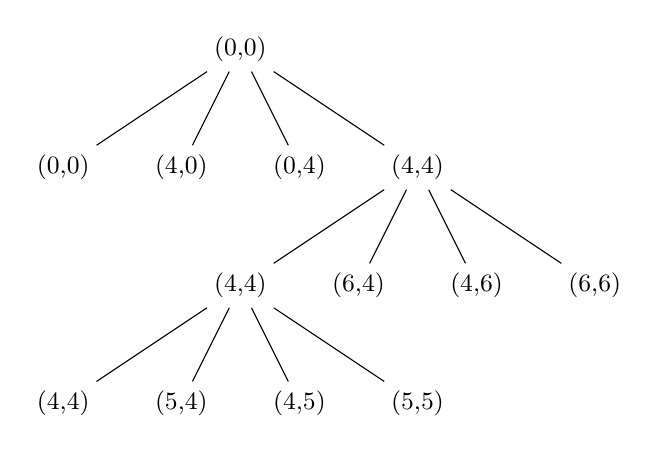
\begin{tikzpicture}[font=\small]
\node {(0,0)}
  child {
    node {(0,0)}
  }
  child {
    node {(4,0)}
  }
  child {
    node {(0,4)}
  }
  child {
    node {(4,4)}
    child {
      node {(4,4)}
      child {
        node {(4,4)}
      }
      child {
        node {(5,4)}
      }
      child {
        node {(4,5)}
      }
      child {
        node {(5,5)}
      }
    }
    child {
      node {(6,4)}
    }
    child {
      node {(4,6)}
    }
    child {
      node {(6,6)}
    }
  };
\end{tikzpicture}
\end{center}
\end{frame}

\begin{frame}{Octrees}
A couple of observations:
\begin{itemize}
\item The height of the node determines the size of the corresponding cube,
      given the size of the topmost, biggest cube.
\item To get the node corresponding to a $(x,y,z)$ coordinate is an 
      $\mathcal{O}(\log n)$ tree search.
\end{itemize} 
\end{frame}

\begin{frame}{Mesh subdivision}
We build the octree from the CSG object by iterative subdivision:
\begin{itemize}
\item Make a queue of cubes, the first one being the root cube.
\item Given the next cube from the queue, how does it relate the objects in 
      the scene?
      \begin{itemize}
      \item It's completely inside of (only) one object: assign the object's 
            material to the cube.
      \item It's on the boundary: subdivide the cube and enqueue the children.
      \end{itemize}
\end{itemize}
Note: this is breadth first. Depth-first is also ok.
\end{frame}

\begin{frame}{Linear octrees}
Memory consumption in the tree representation of octrees is huge:
\begin{itemize}
\item 4/8 bytes for each pointer to children
\item 8 children
\item Millions of nodes
\end{itemize}
\end{frame}

\begin{frame}{Linear octrees}
We need a compact representation.
\begin{itemize}
\item We use a linear octree
\item An array of ordered \emph{location codes} representing the octree's 
      \emph{leaves}
\item Space requirements are greatly reduced by storing only the leaves, 
      without any pointer
\end{itemize}
First introduced by \cite{Gargantini82}.
\end{frame}

\begin{frame}{Linear octrees}
Leaves in the array are stored in traversal order, and identified by their
\emph{location code}:
\begin{center}
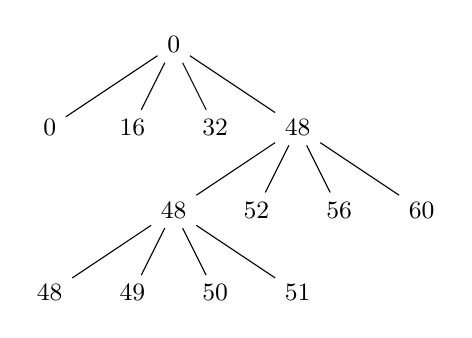
\begin{tikzpicture}[scale=0.7, font=\small]
\node {0}
  child {
    node {0}
  }
  child {
    node {16}
  }
  child {
    node {32}
  }
  child {
    node {48}
    child {
      node {48}
      child {
        node {48}
      }
      child {
        node {49}
      }
      child {
        node {50}
      }
      child {
        node {51}
      }
    }
    child {
      node {52}
    }
    child {
      node {56}
    }
    child {
      node {60}
    }
  };
\end{tikzpicture}
\end{center}
Linear Octree = \{0, 16, 32, 48, 49, 50, 51, 52, 56, 60\}
\end{frame}

\begin{frame}{Location codes}
\begin{itemize}
\item Children of each node in the tree are listed in \emph{Morton order}:
\end{itemize}
\begin{center}
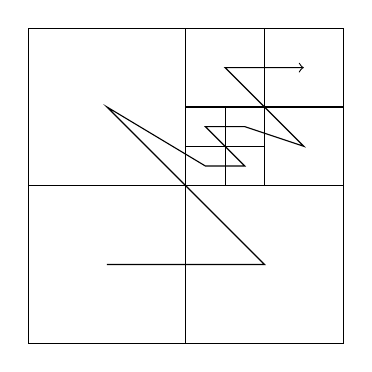
\begin{tikzpicture}[scale=0.5]

\draw (0,0) -- (8,0) -- (8,8) -- (0,8) -- cycle;
\draw (0,4) -- (8,4);
\draw (4,0) -- (4,8);
\draw (4,6) -- (8,6);
\draw (6,4) -- (6,8);
\draw (5,4) -- (5,6);
\draw (4,5) -- (6,5);

\draw [->] (2,2)     -- (6,2)      -- (2,6)      --
           (4.5,4.5) -- (5.5, 4.5) -- (4.5, 5.5) -- (5.5, 5.5) --
           (7,5)     -- (5,7)      -- (7,7);
\end{tikzpicture}
\end{center}
\begin{itemize}
\item So the traversal order of the tree is spatially contiguous 
\item The space-filling curve above is called \emph{Morton curve} 
      \cite{Morton66}
\end{itemize}
\end{frame}

\begin{frame}{Computing Morton codes}
The Morton code of a point in space can be computed from its coordinates very
efficiently by \emph{bit interleaving}.

\begin{equation}
morton(5,4) = morton(\underline{101}, \overline{100}) = 
\overline{1}
\underline{1}
\overline{0}
\underline{0}
\overline{0}
\underline{1} = 49
\end{equation}
To see why, note that while moving through the Morton curve:
\begin{itemize}
\item The $x$ component always changes
\item The $y$ component changes every two steps
\item The $z$ component changes every four steps
\end{itemize}
Note: you have to fix the maximum depth of the tree in advance.
\end{frame}

\begin{frame}[fragile]{Bit interleaving}
How to compute the bit interleaving? Black magic.
\begin{lstlisting}
enum coordinate_t { x = 0, y = 1, z = 2 };

uint64_t morton(uint32_t value, coordinate_t coord)
{
  uint64_t x = value;
  
  x = (x | (x << 32)) & 0xFFFF00000000FFFF;
  x = (x | (x << 16)) & 0x00FF0000FF0000FF;
  x = (x | (x <<  8)) & 0xF00F00F00F00F00F;
  x = (x | (x <<  4)) & 0x30C30C30C30C30C3;
  x = (x | (x <<  2)) & 0x9249249249249249;
  
  return (x << uint8_t(coord));
}
\end{lstlisting}
The only way to get it is doing it on paper and see what happens.
\end{frame}

\begin{frame}{Voxels}
A single cubie in the octree is represented by a 64bits word that we call a 
\emph{voxel}. 

It stores:
\begin{itemize}
\item The morton code of the coordinates
\item The level in the tree (zero at the leaves)
\item Possibly additional data (material of the cube in our application)
\end{itemize}
\end{frame}

\begin{frame}{Voxels}
How to set the size of each field?
\begin{itemize}
\item Decide the precision $p$ for the coordinates, say $p=13$ (bits)
\item The maximum number of cubies in the octree is:
      \begin{equation}
      N=(2^p)^3 = 8^p
      \end{equation}
\item Thus the maximum height of the tree is:
      \begin{equation}
      h_{max} = \log_8 N = p
      \end{equation}
      The maximum height is the number of bits used for the coordinates!
\item We need $\floor{\log_2 h_{max}} + 1$ bits to store the level/height.
\end{itemize}
\end{frame}

\begin{frame}{Voxels}
So we use a 64bits word subdivided by default as follows:
\begin{itemize}
\item $p=13$ bits of precision for each axis \\
      Good enough: a precision of $1mm$ with a range of $10m$
\item $4$ bits to store the level
\item The remaining $21$ bits to store the material of the cube.\\
      Two millions materials are enough in most cases.
\end{itemize}
Can be tuned to have more precision if the number of materials is smaller 
(and probably is).
\end{frame}

\begin{frame}[fragile]{Voxels in the linear octree}
\begin{itemize}
\item Voxels are stored ordered in the linear octree.
\item The morton code is at the most significant bits, the level after it, and 
      the material last.
\item This way the natural ordering of \verb|uint64_t| is what we want:
      \begin{itemize}
      \item To search for a voxel we can compute the morton code of its 
      coordinates and set \emph{level} and \emph{material} to zero. The binary
      search will stop exactly before the position of the voxel.
      \end{itemize}
\end{itemize} 
\end{frame}

\begin{frame}{Tree balancing}
To be useful for successive processing, the mesh must be 
\emph{2-1 edge-balanced}:
\begin{itemize}
\item For each cube, each of its neighbors can be at most 2 times as 
      big (in terms of edge lengths)
\item A cube is considered a neighbor if the two cubes touch on a face or on 
      an edge
\end{itemize}
How to find the neighbors of a cube in the tree?
\end{frame}

\begin{frame}{Linear octree balancing}
Finding the neighbors is done in two steps:
\begin{itemize}
\item Compute the location code of an hypothetical same-size neighbor
      \begin{itemize}
      \item Add the right offset to the coordinates depending on the direction.
      \end{itemize}
\item Search the neighbor in the tree.
      \begin{itemize}
      \item Usual binary search
      \end{itemize}
\end{itemize}
\end{frame}

\begin{frame}{Neighbor location - performance}
What could go wrong?
\begin{itemize}
\item $6 \cdot 4 + 12 \cdot 2=48$ neighbors to find for each cube.
\item $48$ binary searches on a very big array (CPU cache destroyed).
\item Too slow to even think about it.
\end{itemize}
Future solution:
\begin{itemize}
\item Fast algorithm to find the common ancestor of two nodes in the linear 
      octree, provided in \cite{Yoder2006}.
\item Make the binary search collect all the keys in one pass.
\end{itemize}
\end{frame}

\begin{frame}[fragile]{The OcMesh library}
What does the API look like?
\begin{lstlisting}
csg::scene scene;

csg::object *s      = scene.sphere(60);
csg::object *c      = scene.cube(100);
csg::object *body   = intersect(s, c);
csg::object *cavity = scale(0.95, s);
csg::object *result = subtract(body, cavity);

const voxel::material_t metal = 42;

scene.toplevel(result, metal);

octree tree;
tree.build(scene, 0.01);

tree.mesh("/my/mesh/file.obj");
\end{lstlisting}
\end{frame}

\begin{frame}{Future developments}
On the library side (besides the development of the final goal):
\begin{itemize}
\item Improve the CSG expression language
\item Profile and optimize: neighborhood finding, balancing, subdivision
\item Parallelization (easy to do, hard to do really fast)
\end{itemize}
\end{frame}

\section{Bibliography}
\subsection{}
\begin{frame}[allowframebreaks]
\frametitle{Bibliography}
\begin{center}
\bibliographystyle{apalike}
\bibliography{biblio}
\end{center}
\end{frame}

\end{document}
